Im Folgenden wird eine IST-Analyse des Spiels \textit{RimWorld} durchgeführt, um anhand eines Colony Management Games herauszufinden, welche Mechaniken und Eigenschaften dieses Spiel auszeichnen, und welche davon gegebenenfalls übernommen werden könnten für den Prototyp eines neuen Spiels. Dazu wird zu allererst das Spiel näher untersucht, darunter die Mechaniken, die Kernelemente und das User-Interface. Anschließend werden Leitfaden-Interviews durchgeführt, dessen Ergebnisse und Transkripte verwendet werden, um Hypothesen für den Prototypen aufzustellen. Diese Hypothesen werden letztendlich mit einer Umfrage geprüft und mit der Implementierung des Prototypen schlussendlich umgesetzt. 

\subsection{RimWorld}
Das Strategiespiel \textit{RimWorld} ist ein im Jahr 2018 erschienenes Sci-Fi \textit{Colony Management} Game und wurde von \textit{Ludeon Studios} entwickelt und publiziert. Im normalen Szenario startet man mit drei Überlebenden eines Raumschiffabsturzes und versucht seine Kolonie aufzubauen und am Leben zu halten. Das Spiel hat etliche Mechaniken und Tücken, und durch den \textit{AI Storyteller}, welcher eine Vielfalt an Events plant und durchführt, ist eine hohe \textit{replayability} gegeben. Dieser kann auf eine gewünschte Schwierigkeit gestellt werden, von friedfertig bis unfair. Nachdem man den gewünschten Storyteller ausgewählt hat kann man den Planeten generieren (vgl. \autoref{image:rimworld}) und seinen Startpunkt innerhalb der Spielwelt bestimmen (vgl. \autoref{image:rimworld2}).

\begin{figure}
    \begin{center}
        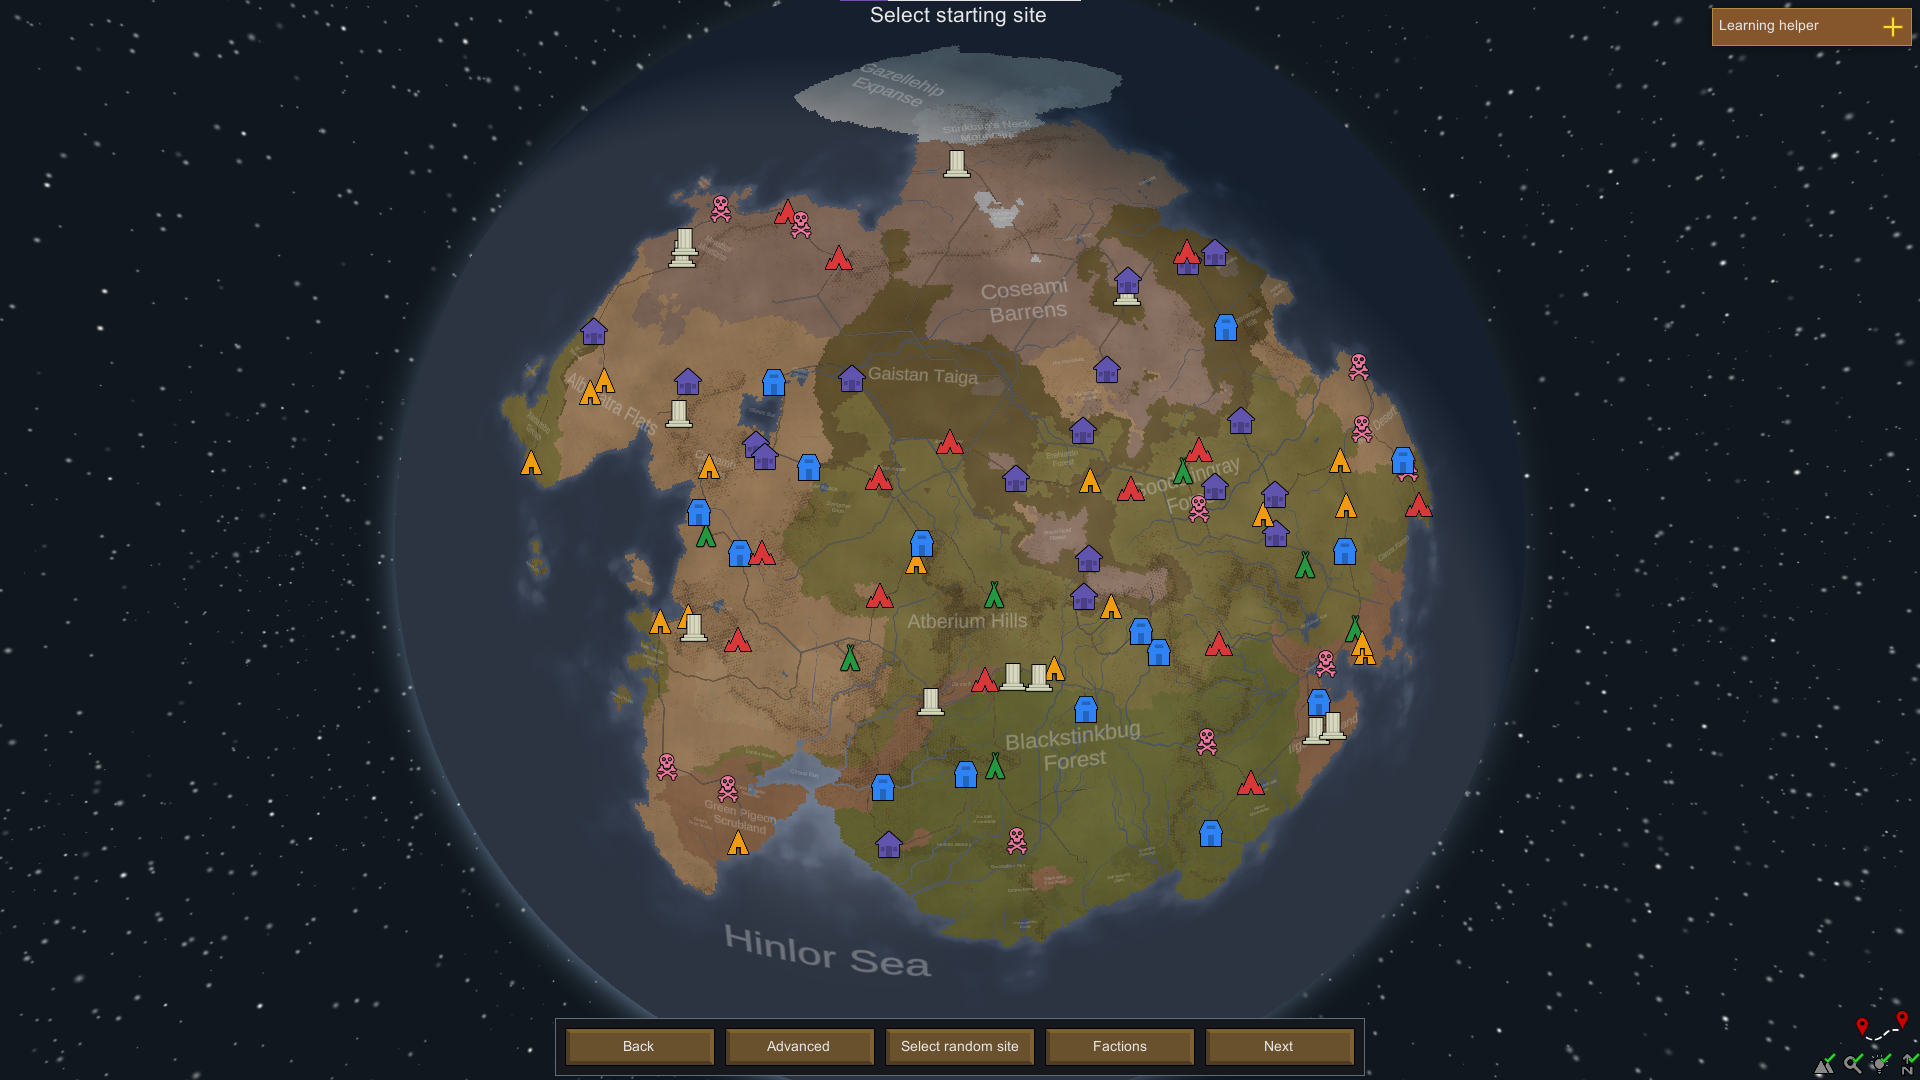
\includegraphics[width=300px]{0.bilder/rimworld.png}
    \end{center}
    \caption{Generierter Planet, Screenshot aus RimWorld} \label{image:rimworld}
\end{figure}

\begin{figure}
    \begin{center}
        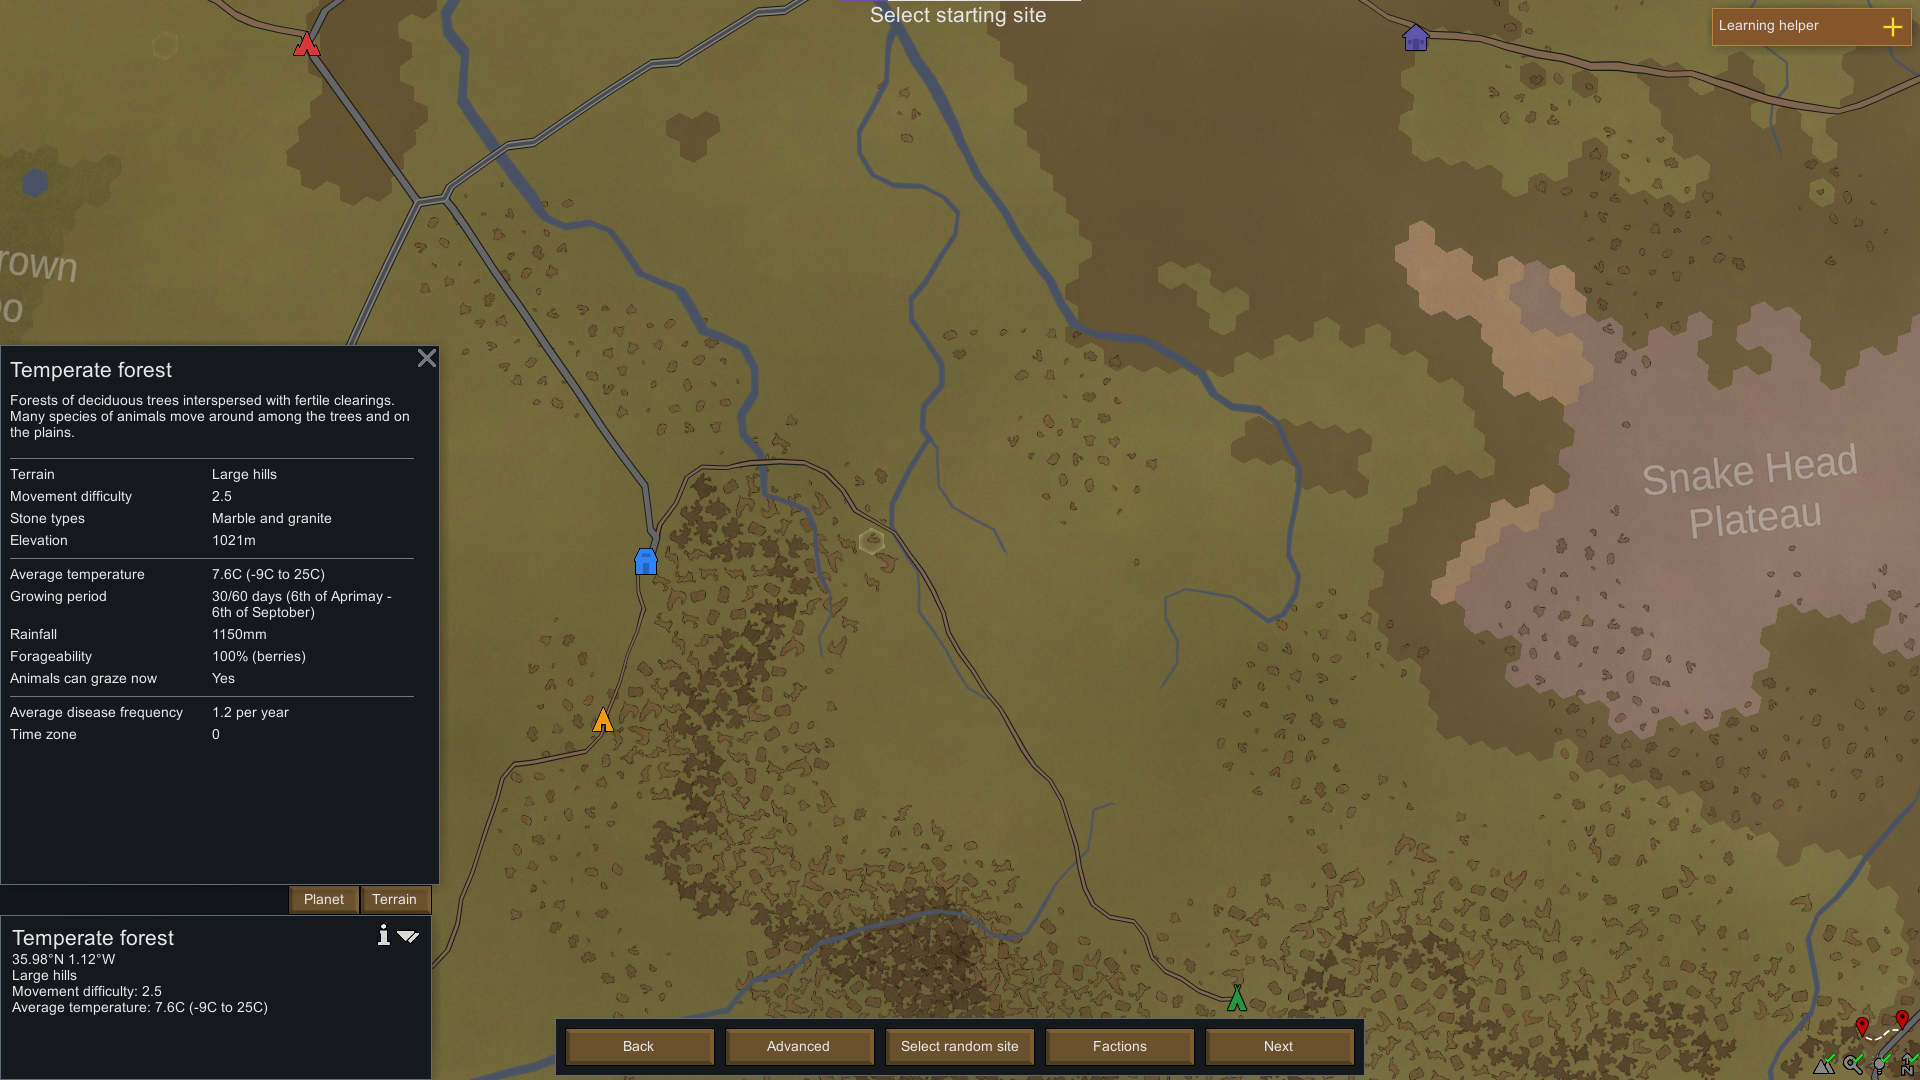
\includegraphics[width=300px]{0.bilder/rimworld2.png}
    \end{center}
    \caption{Ausgewählter Startpunkt für die Kolonie, Screenshot aus RimWorld} \label{image:rimworld2}
\end{figure}

\newparagraph{Spielwelt}
Die Welt ist für gewöhnlich eine Pangaea-artige Landmasse auf einem dreidimensionalen, blauen Planeten mit einem Äquator und einem Pol (vgl. \autoref{image:rimworld}). Der Planet ist aufgeteilt in hexagonale Kacheln, welche jeweils eine Karte symbolisieren. Die Kacheln haben dabei jeweils verschiedene Eigenschaften, die dann auf der gesamten Karte, welche der Spieler aussucht, gelten. Auf \autoref{image:rimworld2} lassen sich am linken Rand die meisten Eigenschaften anzeigen. Darunter die Terrain-Eigenschaften, wie viel Berge es gibt und damit auch Erzquellen, welche Steinarten es gibt und die Höhe der Karte. Außerdem ist ein maßgeblicher Faktor die Extreme der Temperaturen, zu welchen Zeiten man Felder anbauen kann und wie viel Regen für gewöhnlich fällt. Der Name der Kacheln, in diesem Fall \glqq Temperate Forest\grqq, gibt außerdem Aufschluss darüber, wie bewaldet die Kachel ist. Je nach Distanz zum Pol oder Äquator ändern sich diese Eigenschaften. Außerdem besitzen manche Kacheln einen Fluss oder bestehen gänzlich aus Wasser oder Eis, oder haben eine Anbindung zu einer Straße (grau) oder einem Feldweg (braun). Wählt man eine Kachel aus und drückt auf \glqq Next\grqq\;am unteren Bildschirmrand, gelangt man in die Auswahl der Kolonisten.

\newparagraph{Kolonisten}
Das Herz des Spielgeschehens sind die Kolonisten, die, mit manchen Ausnahmen, ihre zugewiesenen Aufgaben erfüllen. Die drei Startkolonisten kann man so lange neu generieren, bis man zufrieden ist. Es gibt dabei mehrere Eigenschaften, die ein Kolonist mit sich bringt. Die darunter fundamentalsten Eigenschaften sind die \textit{Skills}, welche mittig in \autoref{image:rimworldcharacter} zu sehen sind. Es gibt 12 verschiedene Skills, wovon jeder Kolonist ein bestimmtes Level hat. Diese werden zwischen \textit{0 - 5} generiert, wonach noch die \textit{Hintergründe} (engl. \textit{backstories}) und \textit{Eigenschaften} (engl. \textit{traits}) der jeweiligen Kolonisten addiert werden \cite*[]{rimworld:colonist}. Manche Hintergründe addieren oder subtrahieren Level von Skills, manche machen manche Tätigkeiten und damit einhergehende Skills auch unmöglich, darunter der Hintergrund \textit{Romanschriftsteller} (engl. \textit{novelist}), welcher es dem Kolonisten unmöglich macht, einfache Arbeiten zu erledigen, etwa Putzen oder Gegenstände umhertragen \cite*[]{rimworld:backstories}. Eigenschaften sind analog zu den Hintergründen zufällig generiert, beziehen sich größtenteils jedoch auf soziale Interaktionen oder bringen bestimmte Boni oder Mali für die \textit{Stimmung} des Kolonisten, darunter Sexualitäten, wie schnell der Kolonist lernen kann, oder exotischere Eigenschaften wie \textit{Kannibale} oder \textit{Psychopath} \cite*[]{rimworld:traits}. Die Flammen neben dem Level der Skills stehen für die \textit{Passion} des Kolonisten für bestimmte Skills. Ist keine Flamme neben dem Level zu sehen, so lernt der Kolonist diese Fähigkeit beim Durchführen davon mit einem Faktor von \textit{35\%}. Ist eine Flamme vorhanden, ist der Kolonist \textit{interessiert} und hat einen Lernfaktor von \textit{100\%}. Sind zwei Flammen vorhanden, \textit{brennt} der Kolonist für diese Tätigkeit und lernt mit einem Faktor von \textit{150\%}. Da viele verschiedene Tätigkeiten zu bestimmten Zeitpunkten ausschlaggebend für das Überleben der Kolonie sein könnten, kann es sinnvoll sein, eine breite Palette verschiedener Passionen und hochrangigen Skills zu haben. Ältere Kolonisten haben für gewöhnlich höhere Skills, sind jedoch davon öfter von \textit{Gesundheitsproblemen} betroffen, etwa Verlust von Seh- und Hörvermögen, oder langsamere Laufgeschwindigkeit. Außerdem haben manche Startkolonisten bereits zuvor gebildete \textit{Beziehungen} zu manch anderen, welche bestimmte Interaktionen vereinfachen oder erschweren.
 
\begin{figure}
    \begin{center}
        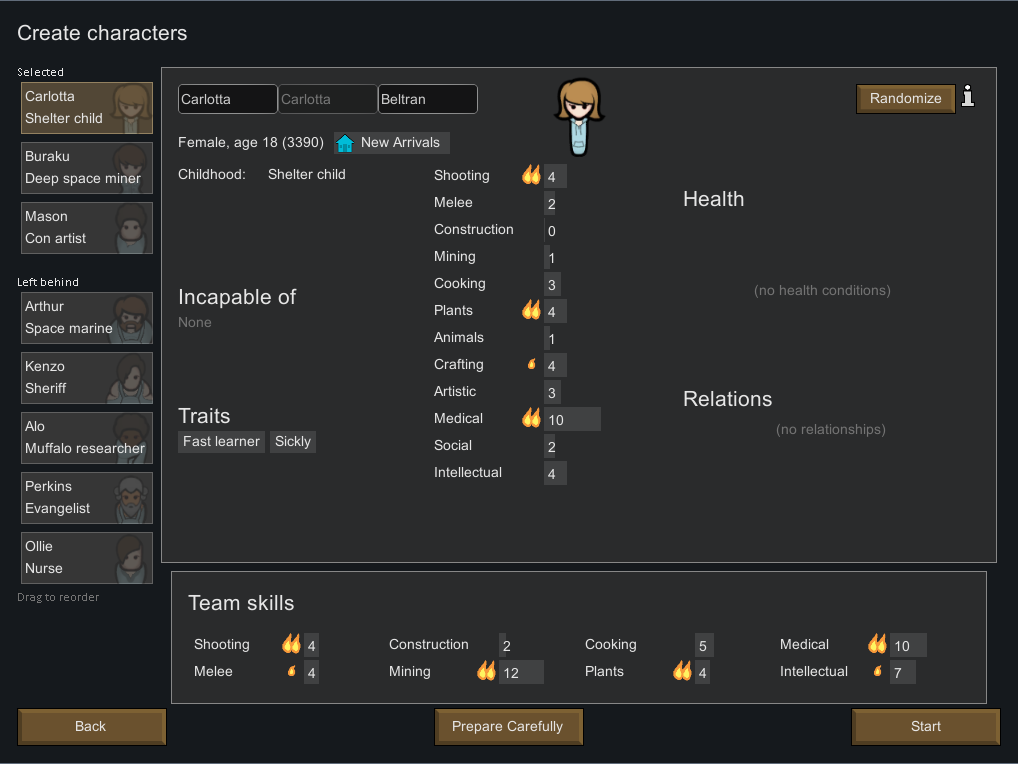
\includegraphics[width=300px]{0.bilder/rimworldcharacter.png}
    \end{center}
    \caption{Auswahl der Startkolonisten, Screenshot aus RimWorld} \label{image:rimworldcharacter}
\end{figure}

\newparagraph{Spielgeschehen}
Der Spieler wird nach der Anfangssequenz des Absturzes der Kolonisten nicht an die Hand genommen. Ein großer Teil des Spieles besteht darin, Strategien für das Überleben der Kolonie zu finden. Für gewöhnlich beginnt man damit, erste Teile der zukünftigen Basis zu bauen, wie diese aussehen soll und aus welchem Material diese besteht ist, wie so oft in diesem Spiel, dem Spieler selbst überlassen. Jeder Kolonist hat eine \textit{Stimmung} (engl. \textit{mood}), welche es gilt im Auge zu behalten (vgl. \autoref{image:rimworldmood}). Sollte die Stimmung zu lange zu niedrig sein, wird der Kolonist in einen nicht kontrollierbaren Zustand fallen, auch engl. \textit{mental break} genannt, wovon es verschiedene gibt. Darunter \textit{tantrum}, wobei der Kolonist alle möglichen Gebäude und Strukturen in seiner Sichtweite attackiert und möglicherweise zerstört, oder \textit{given up and leaving}, wobei der Kolonist die Spielerkolonie verlässt und aus dem Spiel entfernt wird \cite*[]{rimworld:mentalbreak}. Um diese Zustände zu vermeiden muss der Spieler sinnvoll die zu Anfang gegebenen Ressourcen nutzen, und für Nahrung, Unterschlupf, Wärme, Licht und etliche weitere Gegebenheiten sorgen. Je nach gewählten AI Storyteller passieren selten oder öfter Events, welche das Spielgeschehen maßgeblich beeinflussen können. Darunter sind \textit{raids}, wobei fremde Kolonien die Spielerkolonie angreifen, Gebäude zerstören, Reichtümer stehlen oder Kolonisten verschleppen, oder ein zufälliger Ansturm an Biebern, welche sämtliche Bäume auf der Karte Stück für Stück abholzen \cite*[]{rimworld:events}. Um gegebene Probleme zu Lösen kann der Spieler neue Technologien erforschen, welche letztendlich bis zum Bau eines Raumschiffes führen, was das vorprogrammierte Endziel des Spiels ist. Auf dem Weg zum Bau des Raumschiffes wird der Spieler also konstant vor neue Probleme, Launen der Kolonisten und Ressourcenmanagement gestellt, wodurch eine hohe replayability gegeben ist.

\begin{figure}
    \begin{center}
        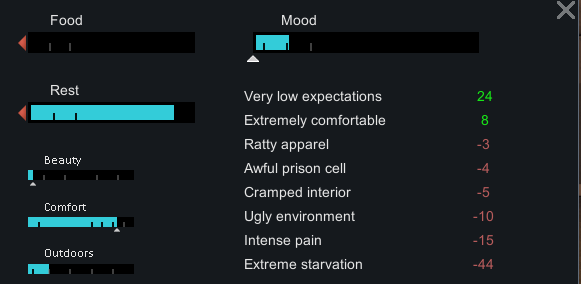
\includegraphics[width=300px]{0.bilder/rimworldmood.png}
    \end{center}
    \caption{Stimmungsbalken und -einflüsse, Screenshot aus RimWorld} \label{image:rimworldmood}
\end{figure}

\newparagraph{User Interface}
Das UI von RimWorld ist recht gefüllt, denn in jeder Ecke des Bildschirms finden sich direkt mehrere verschiedene Informationen, welche der Spieler erst kennenlernen und verstehen muss. Im Folgenden wird sich stark auf \autoref{image:rimworldui} berufen, anhand dessen das UI analysiert wird. Das UI ist zum besseren Verständnis in 13 verschiedene Stücke aufgeteilt, welche allesamt eigene Funktionen und einen bestimmten Mehrwert bieten. 

\begin{figure}
    \begin{center}
        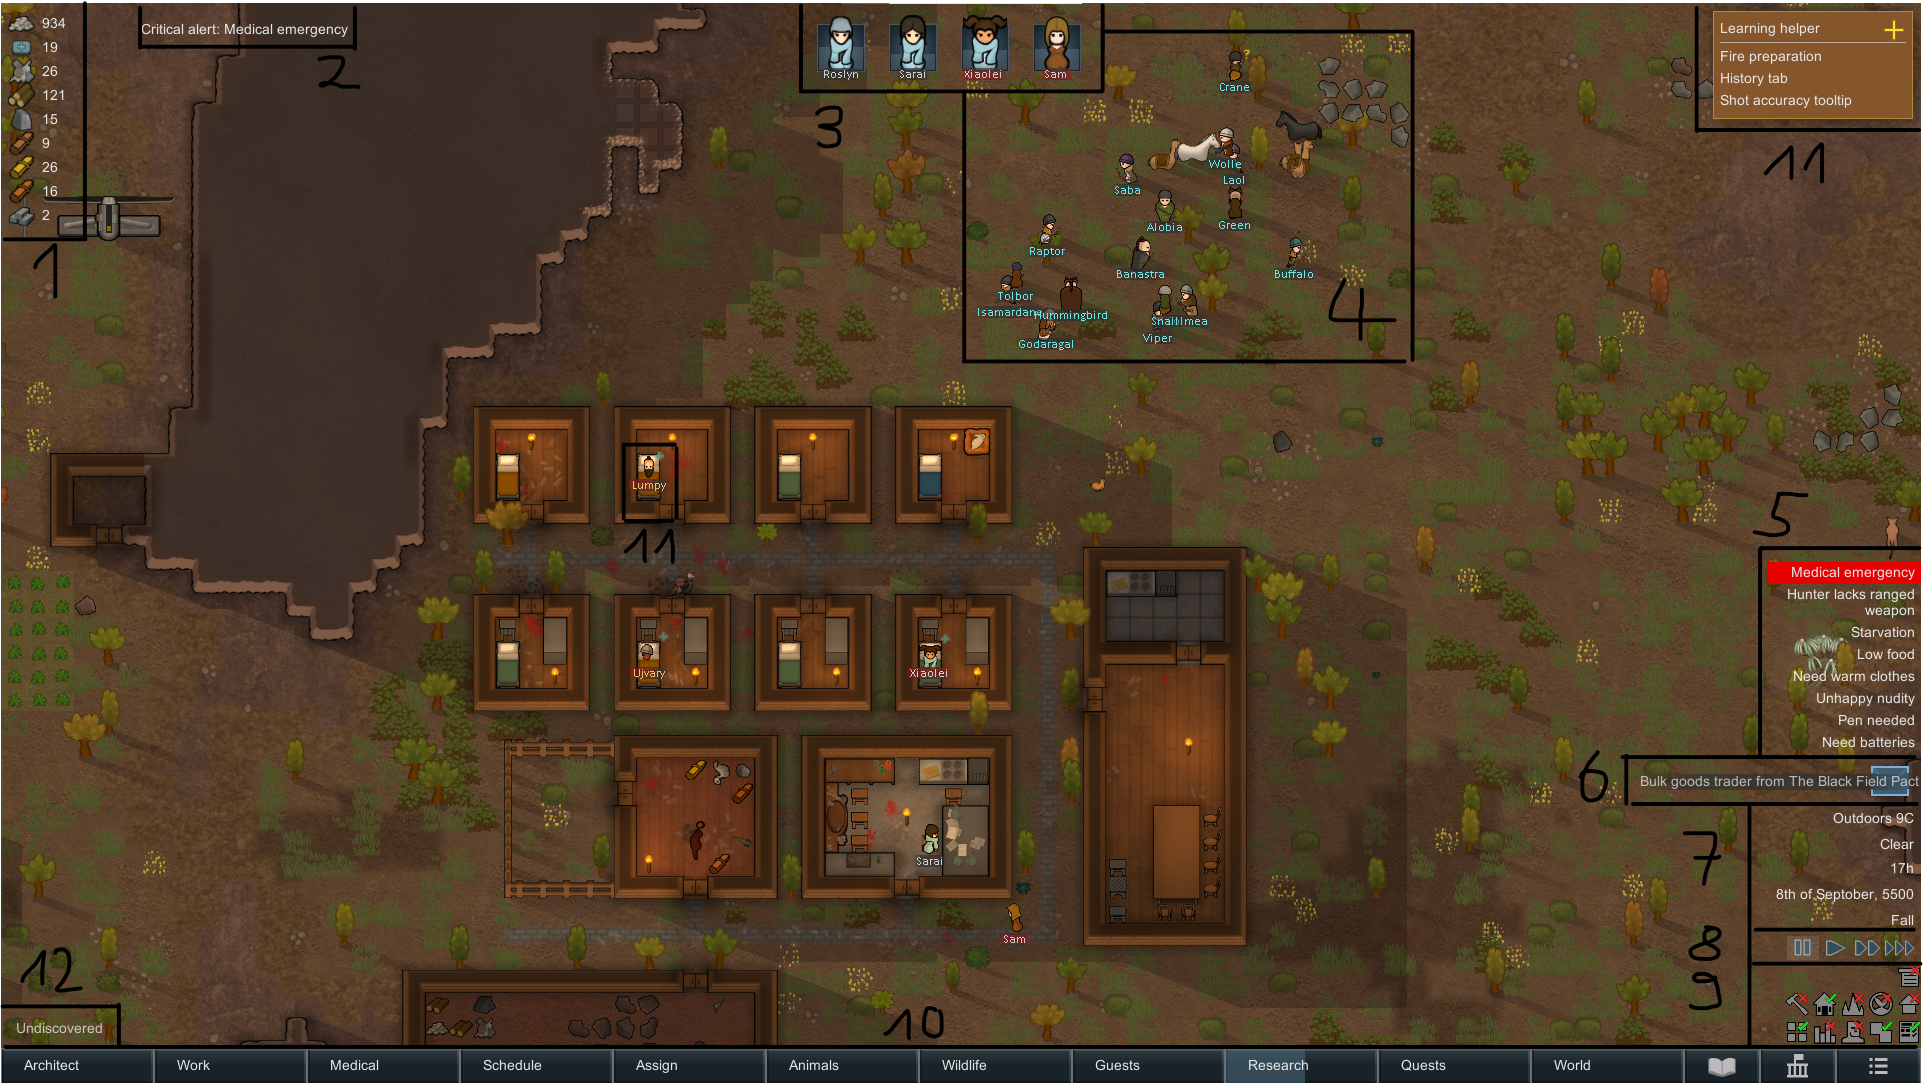
\includegraphics[width=400px]{0.bilder/rimworldui.png}
    \end{center}
    \caption{User Interface, Screenshot aus RimWorld} \label{image:rimworldui}
\end{figure}

Der erste Bereich des UI (1) zeigt die Ressourcen im Besitz des Spielers. Nicht alle Ressourcen werden vom Spieler besessen, sondern erst jene, die im definierten Lager vorhanden sind.
Der zweite Bereich (2) ist für kritische Meldungen, die sofortiges Handeln erfordern, in diesem Fall ein medizinischer Notfall, welcher zum Tod des Kolonisten führen kann.
In Bereich (3) werden alle Kolonisten, die Teil der eigenen Kolonie sind, angezeigt. Man kann dort sowohl Namen, als auch Aussehen, derzeitige Lebenspunkte und momentane Stimmung ablesen (hellblaue Füllung im Hintergrund des Quadrats).
Im vierten Bereich (4) ist gerade ein Event zu sehen, welches zufällig generiert wurde. In diesem Fall wird die Spielerkolonie von einer Händlerkarawane besucht, welche ein eigenes Inventar hat und mit dem Spieler handeln kann, also auch ein \textit{Händler} im Sinne einer ökonomischen Funktion.
Bereich (5) zeigt einige Zustände der Spielerkolonie an, darunter derzeitig hungernde Kolonisten, oder dass ein Jäger keine Waffe zum Jagen besitzt. Sehr dringende Zustände mit sofortigem Handlungsbedarf werden, wie in der Grafik zu erkennen, rot hinterlegt dargestellt.
In Bereich (6) werden ausschließlich vom AI Storyteller generierte Events mitgeteilt, also Hitzewellen, Angriffe oder, wie in diesem Fall, Besuche von Händlerkarawanen.
Im siebten Bereich (7) erkennt man meteorologische Informationen zu derzeitigen Wettergegebenheiten, der Temperatur, den derzeitigen Monat und die Jahreszeit.
Bereich (8) beinhaltet die Elemente zur Steuerung der Spielgeschwindigkeit.
Bereich (9) zeigt verschiedene Optionen zum Anzeigen bestimmter Informationen. Man kann sich beispielsweise noch die Fruchtbarkeitsgrade des Bodens einblenden lassen, oder die Schönheit der Umgebung aus der Sicht eines Kolonisten.
Der zehnte Bereich (10) stellt die Menüleiste dar, unter welcher man die meisten Aktionen im Spiel durchführen kann. Unter dem Reiter \textit{Architect} finden sich zum Beispiel Möbel und Strukturen (vgl. \autoref{image:rimworlduimenu}), welche man platzieren kann. Der am besten passende Kolonist wird dann dieser Tätigkeit zugeordnet. Bereich (11) zeigt einen im Bett liegenden Kolonisten, welcher zuvor verwundet wurde und sich nun regeneriert. Bereich (12) zeigt Informationen über das Element, auf welche die Maus gerade liegt. Dort können interessante Informationen bereitgestellt werden, zum Beispiel auf dem Boden befindlicher Dreck oder Blut, welches aufgeräumt werden sollte. Der letzte, nicht markierte Bereich ist der restliche Bereich des Bildschirms, wo sämtliches Spielgeschehen simuliert wird. Man erkennt den Anfang einer Kolonie, bestehend aus einigen Holzbaracken, einer Küche, einem Raum mit Tisch, um dort zu essen, ein kleines Lager und einen Produktionsraum, wo die Kolonisten die meiste ihrer Arbeit verrichten.

\begin{figure}
    \begin{center}
        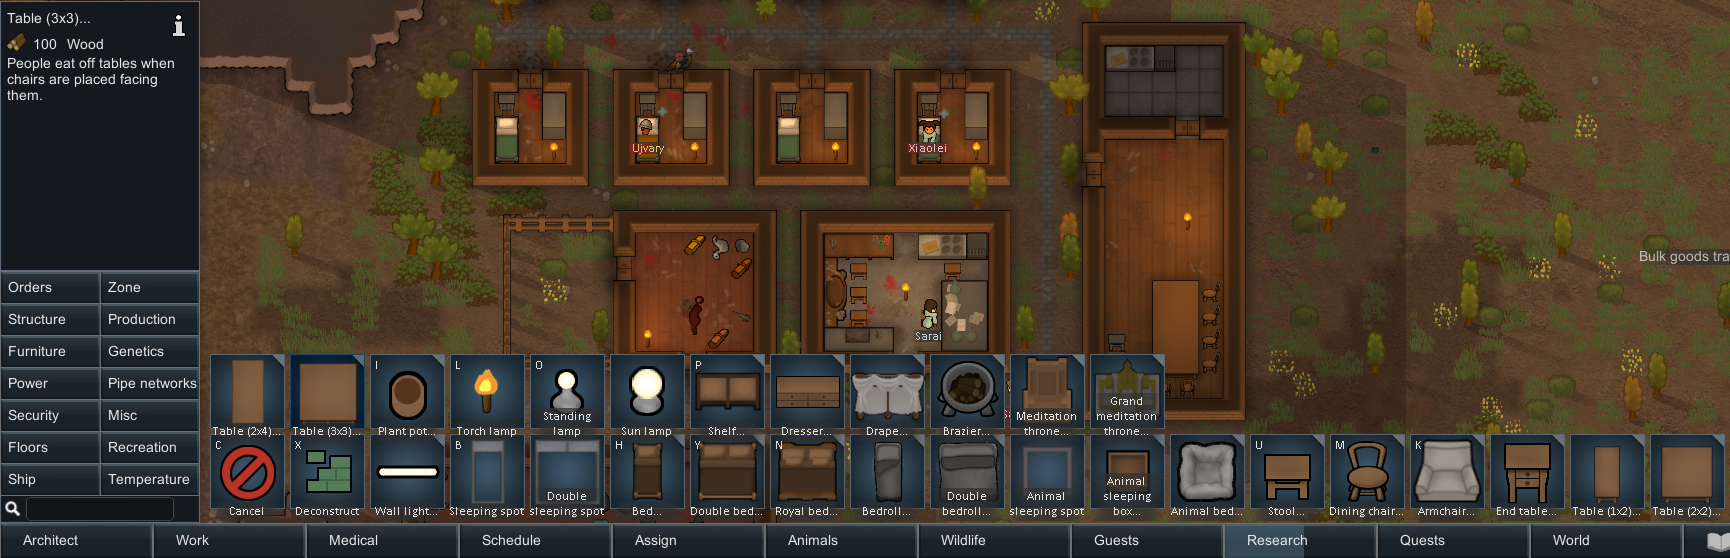
\includegraphics[width=400px]{0.bilder/rimworlduimenu.png}
    \end{center}
    \caption{Baumenü, Screenshot aus RimWorld} \label{image:rimworlduimenu}
\end{figure}

\newparagraph{Prioritäten}
Ein Großteil des Spielgeschehens läuft über die Prioritäten der Kolonisten. Man kann für jegliche mögliche Tätigkeit eine manuelle Priorität setzen (vgl. \autoref{image:rimworlduipriorities}), wodurch die Kolonisten erst bestimmte Tätigkeiten verrichten, bevor manch andere angefangen werden. Die Prioritäten reichen dabei von \textit{4} - niedrige Priorität, bis \textit{1} - hohe Priorität. Durch Linksklick auf ein Prioritätenfeld erhöht man die Priorität, durch Rechtsklick erniedrigt man sie. Man kann ebenfalls die Priorität auf \textit{nichts} setzen, wodurch die Tätigkeit unter keinen Umständen ausgeführt wird. Es kann daher sinnvoll sein, die Prioritäten höher zu setzen bei überlebenswichtigen Dingen wie Feuerlöschen oder medizinischer Hilfe, falls darin geübt.
\begin{figure}
    \begin{center}
        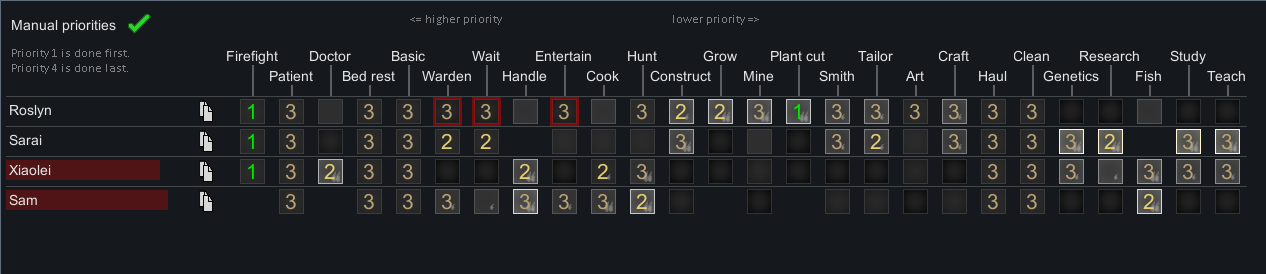
\includegraphics[width=400px]{0.bilder/rimworlduipriorities.png}
    \end{center}
    \caption{Prioritäten, Screenshot aus RimWorld} \label{image:rimworlduipriorities}
\end{figure}

\newparagraph{Steuerung der Kolonisten}
Anders als traditionelle Resource Management Games (Age of Empires, Civilization), steuert man seine Einheiten nicht \textit{direkt}, in dem man diese auswählt und dann auf das gewünschte Feld klickt, sondern \textit{indirekt}. Man wählt zuerst die auszuführende Tätigkeit aus der Liste der möglichen Befehle aus (vgl. \autoref{image:rimworldorders}), markiert den Bereich für den Befehl und der nächstbeste Kolonist, der diese Aufgabe erfüllen kann und die höchste Priorität dafür hat, wird zugewiesen sich darum zu kümmern. Das macht die zuvor genannten Prioritäten unerlässlich, um einen reibungslosen Spielverlauf zu haben. Der Vorteil dieser Mechanik ist ganz klar, dass sich das Management der Kolonisten eher anfühlt wie das einer Ameisenkolonie, statt dem herkömmlichen direkten Kommandieren der einzelnen Einheiten. Der klare Nachteil davon ist, dass man nicht immer die gewünschten Dinge erledigen lassen kann, die man gerade hätte. In manchen Situationen sind andere Tätigkeiten prioritär, wodurch man die Prioritäten stetig im Auge behalten muss und öfter mal anpasst, sodass auch wirklich das erledigt wird, was gerade notwendig ist.

\newparagraph{Ressourcen}
Das Spiel hat eine große Vielfalt an verschiedener Ressourcen. Darunter fallen Grundbedarfsgüter, wie eine einfache Mahlzeit, Heu oder Reis. Es gibt von einigen Rohstoffen allerdings verschiedenste Ausführungen, so hat beispielsweise Leder \textit{20} verschiedene Variationen (Schweinehaut, Hundeleder, Fuchsfell, \dots). Es gibt weiterhin sehr exotische Güter, zum Beispiel verschiedene bionische Körperteile, mit welchen man fehlende ersetzen kann, oder Nanobots, die fehlende Organe wiederherstellen können \cite*[]{rimworld:resources}. Es gibt eine Vielfalt an verschiedener, zubereitbarer Mahlzeiten, welche verschiedene Boni auf die Stimmung geben und jeweils verschiedene Rohstoffe benötigen.


\begin{figure}
    \begin{center}
        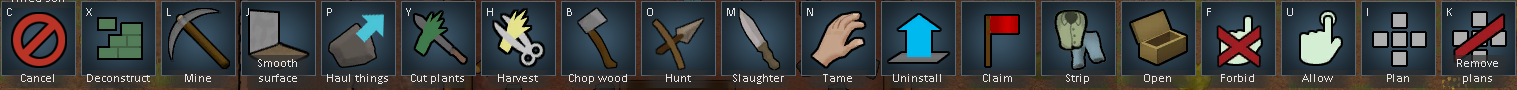
\includegraphics[width=400px]{0.bilder/rimworldorders.png}
    \end{center}
    \caption{Befehle, Screenshot aus RimWorld} \label{image:rimworldorders}
\end{figure}

\newparagraph{Haltbarkeiten}
Viele greifbare Ressourcen, welche auch in der realen Welt aufgrund von Korrosion zerstört würden oder als Lebensmittel mit der Zeit ablaufen, besitzen eine Haltbarkeit. Diese sinkt stetig mit vergehender Zeit von 100 auf 0. Ist diese auf 0 gesunken, verschwindet die Ressource aus dem Spiel, damit stellt diese Mechanik der Haltbarkeit ein Drain dar. Manche Ressourcen benötigen ein Dach oder einen Raum, damit die Haltbarkeit nicht weiter sinkt, andere wiederum und darunter primär Lebensmittel, benötigen eine sehr niedrige Temperatur, damit sie konserviert werden können.


\begin{figure}
    \begin{center}
        
\includegraphics[width=400px]{0.bilder/interviewphases.png}
    \end{center}
    \caption{Die Vier Phasen des Interviews} \label{image:interviewphases}
\end{figure}
\subsection{Interviews}
Für die Ermittlung gut funktionierender Mechaniken und Konzepte wird auf die Methode der nutzungsorientierten Gestaltung des kontextuellen Interviews zurückgegriffen \cite*[]{holtzblatt_beyer_1997}. Dazu wird ein Leitfadeninterview angefertigt, um qualitative Daten von den Teilnehmern zu extrahieren und daraus Hypothesen anzufertigen \cite*[]{baur_blasius}. Nachdem die Hypothesen erarbeitet wurden, werden diese mittels einer Umfrage in einem breiten Umfang überprüft. Es werden drei Personen ausgewählt, wobei die Erfahrung aller Personen in Bezug auf das Spiel und das Genre generell variiert. Diese Personen, im Folgenden auch \textit{Probanden} genannt, werden in Einzelgesprächen dazu gebeten, dass Spiel eine Stunde lang zu spielen. Einzelgespräche beziehungsweise -interviews sind Gruppengesprächen vorzuziehen, da die einzelnen Probanden einen entspannteren Zeitplan haben, sich gänzlich auf das Spiel und die Fragen fokussieren können und keine Gefahr laufen, abgelenkt zu werden oder mit anderen Probanden in Gespräche zu gelangen \cite*[]{lankoski_bjork}. Das Interview gliedert sich in vier Phasen (vgl. \autoref{image:interviewphases}).

\subsubsection{Versuchsaufbau}
Im Zentrum des Interviews steht, neben den Einleitungs- und Abschlussfragen, das Videospiel \textit{RimWorld}, welches für eine Stunde lang von den Probanden gespielt wird. Das Spiel läuft zu dem Zeitpunkt der Interviews auf der Version \textit{1.3.3387}, ist auf die englische Sprache eingestellt und wird über die Online-Vertriebsplattform für Computerspiele \textit{Steam} ausgeführt.
Das Interview ist, wie bereits erläutert, in vier Phasen gegliedert und wird in der Wohnung des Interviewers durchgeführt. Wichtig ist, dass alle Probanden leicht andere Qualifikationen besitzen, sodass ein breites Bild über den Zustand des untersuchten Spiels erstellt werden kann. Es ist fundamental zu erkennen, wie ein Spiel von Kennern, wie auch von Neulingen empfunden wird. Jedes Interview wird dabei mit einem Mikrofon aufgenommen und anschließend transkribiert. Die Transkripte sind wörtlich und nicht lautsprachlich angefertigt. Dies bietet den einfachen Vorteil, dass die später aufgestellten Hypothesen mit Textbelegen der Aussagen der jeweiligen Teilnehmer aufgestellt beziehungsweise belegt werden können. Allerdings werden die Namen der Teilnehmer nicht genannt und stattdessen durch ein Pseudonym ersetzt \cite*[S.97]{lankoski_bjork}. Alle angefertigten Transkripte sind im Anhang auffindbar, wovon für den kommenden Abschnitt \hyperref[transcript:A]{Transkript A}, \hyperref[transcript:B]{Transkript B} und \hyperref[transcript:C]{Transkript C} relevant sind.
 
\newpage
\paragraph {Einleitung}
Um die erhobenen Daten richtig kategorisieren zu können, werden als erstes grundlegende Daten zu der Person an sich erfasst:
\begin{itemize}
    \item F1: Wie alt bist du?
    \item F2: Nach welchem Geschlecht identifizierst du dich?
\end{itemize}

\paragraph{Aufwärmen}
Im zweiten Schritt des Interviews werden etwas spezifischere Fragen zu der Erfahrung und dem Verhalten bezüglich Videospielen gestellt:
\begin{itemize}
    \item F3: Hast du bereits Erfahrung in Videospielen?
    \item F4: Hast du bereits Erfahrung in Resource Management Games?
    \item F5: Hast du RimWorld bereits zuvor gespielt?
\end{itemize}

\paragraph{Beobachtung}
Die Phase der Beobachtung beschreibt die Spielphase. Der Proband wird dazu aufgefordert, das Videospiel \textit{RimWorld} zu spielen. Es ist von fundamentaler Wichtigkeit für diese Phase, das die beobachtende Person keinerlei Versuch unternimmt, sich in das Spielgeschehen oder das Verhalten der beobachteten Person einmischt. Es wird auch unterlassen, begangene Fehler aufzuklären oder in irgend einer anderen Art und Weise zu helfen, falls nicht anders möglich. Außerdem ist es wichtig zu erwähnen, dass nicht alle Fragen zwangsweise gestellt werden. Diese Fragen dienen lediglich als Katalog möglicher Fragen, die situativ gestellt werden können.

\begin{itemize}
    \item F6: Welche Emotion wird gerade verspürt?
    \item F7: Ist das Spiel für den Probanden immersiv?
    \item F8: Hat der Proband Verlustängste bezüglich der Kolonisten?
    \item F9: Wieso machst du \_\_\_?
    \item F10: Weißt du, was du nun tun kannst?
    \item F11: Was ist dein nächstes Ziel?
    \item F12: Verwendet der Proband die Prioritätenliste?
    \item F13: Kommt der Proband gut mit der indirekten Anweisungsmechanik zurecht?
\end{itemize}

\paragraph{Abschluss}
In der Abschlussphase wird der Proband gebeten, eine eigene Meinung abzugeben. Außerdem können Fehler aufgeklärt werden und inhaltliche Fragen beantwortet werden, ohne dass sie nun das Verhalten im Spiel verzerren.

\begin{itemize}
    \item F14: Was hast du als gut empfunden?
    \item F15: Was hast du als schlecht empfunden?
    \item F16: Wie findest du das indirekte Anweisen?
    \item F17: Was sagst du zu der Ressourcenvielfalt?
    \item F18: Was hältst du von dem Prioritätensystem?
    \item F19: Wie findest du die vielen zufällig generierten Umstände?
\end{itemize}

\subsubsection{Probanden}
Für die Interviews werden exakt drei Personen ausgewählt, welche sich allesamt in ihrer Erfahrung in Videospielen und auch in ihrer Erfahrung in RimWorld unterscheiden. Es ist damit zu erhoffen, dass ein möglichst breites Spektrum an Informationen extrahiert werden kann. Da Proband C sich zu dem Zeitpunkt des Interviews nicht vor Ort befand, wurde mit dieser Person stattdessen über Discord ein Meeting gehalten, in welchem der Bildschirm des Probanden dem Interviewer geteilt wurde. Der Prozess lief unwesentlich unkomplizierter ab, da beide Personen bereits vertraut mit der Software waren. 

% Please add the following required packages to your document preamble:
% \usepackage{graphicx}
\begin{table}[]
    \centering
    \caption{Jeweilige Antworten der Probanden auf die Einleitungsfragen}
    \label{table:interview}
    \begin{tabular}{|l|c|c|c|}
    \hline
                                  & Proband A & Proband B & Proband C \\ \hline
    Alter                         & 19        & 23        & 24        \\ \hline
    Geschlecht                    & \female        & \male         & \male        \\ \hline
    Erfahrung Videospiele         & $\upchi$      & \checkmark        & \checkmark        \\ \hline
    Erfahrung Resource Management & $\upchi$      & \checkmark        & \checkmark       \\ \hline
    Erfahrung RimWorld            & $\upchi$      & $\upchi$      & \checkmark       \\ \hline
    \end{tabular}
    \end{table}

\subsubsection{Ablauf}
Jegliches Interview beginnt mit den Einleitungsfragen, wobei die Antworten der Probanden zusammengefasst in \autoref{table:interview} zu finden sind. Die Altersspanne der Teilnehmer liegt zwischen 19 und 24 Jahren, mit einem Altersdurchschnitt von 22 Jahren. Zwei der drei Probanden sind männlich, ein Teilnehmer ist weiblich. Die beiden männlichen Teilnehmer weisen beide bereits Erfahrung in Videospielen und Resource Management Games auf, wobei lediglich einer der beiden männlichen Teilnehmer bereits RimWorld zuvor gespielt hat. Alle Teilnehmer wurden darüber in Kenntnis gesetzt, dass ihre Stimmen aufgezeichnet werden, und waren damit einverstanden. Die im Folgenden aufgestellten Hypothesen werden mit [HX] gekennzeichnet, wobei das X eine fortlaufende Nummerierung der jeweiligen Hypothesen darstellt. Die Referenzen auf die Transkripte werden mit [X, Z.Y] dargestellt, wobei X in diesem Fall das Pseudonym des jeweiligen Probanden ist (A, B, C), und Y die jeweilige Zeile in dem gegebenen Transkript.

Zu Beginn fällt auf, dass der Startbildschirm des Spiels sehr viele Buttons enthält, und die Option \glqq New Colony\grqq für Neulinge nicht unbedingt eindeutig assoziiert wird mit dem Beginn eines neuen Spiels [A, Z.27-30]. Es wäre daher sinnvoll, die Anzahl der Knöpfe auf ein Minimum zu reduzieren [H1]. Die Steuerung und die einzelnen Symbole auf der generierten Weltkarte sind nicht eindeutig assoziierbar [A, Z.39-48][B, Z.38-54], eine gewisse, gut sichtbare Erklärung oberhalb der Weltkugel wäre eine hilfreiche Ergänzung [H2]. Für spezielle, stark herausfordernde Gegner oder Umgebungseigenschaften empfiehlt sich die Möglichkeit, diese auch ausstellen zu können [H3]. Das gibt dem Spieler mehr Kontrolle über mögliche Frustration [C, Z.37-40]. Außerdem fällt auf, dass, gerade für Neulinge, die englische Sprache in Videospielen etwas speziell sein kann. Diese Spiele enthalten Begriffe, welche im schulischen oder alltäglichen Kontext eher weniger auftreten und daher erst gelernt werden müssen. Es ist daher sinnvoll, möglichst viele Sprachen aufgrund der höheren Inklusion und den dadurch niedrigeren Frust zu implementieren [H4][A, Z.49]. Die Auswahl der Startkachel hängt scheinbar sehr stark mit der Erfahrung des Probanden zusammen, Proband A wählt den Startpunkt zufällig [A, Z.41-48], um möglichst schnell das eigentliche Spiel zu beginnen, während Proband B den Startpunkt abhängig von den benachbarten Fraktionen macht, da diese als positiv assoziiert werden [B, Z.56-59]. Proband C ist der einzige Proband, welcher sich die Eigenschaften der einzelnen Kachel anschaut und basierend auf konkreteren Informationen die Entscheidung fällt, darunter die Anbauzeit und die Terrain-Beschaffenheit [C, Z.43-44]. Dieser Lernprozess und die damit verbundene, gewonnene Erfahrung, ist nicht schlecht. Es lässt Raum für Verbesserung und Lerneffekte. Dem Spieler sollte daher nicht mitgeteilt werden, welche Kacheln sinnvoller wären, als andere [H5]. In der Auswahl der Kolonisten fällt auf, dass selbst Spieler, welche bereits Erfahrung in anderen Spielen des Genres haben, leicht überfordert mit der Anzahl und Diversität der Eigenschaften der Kolonisten haben können [B, Z.74-77]. Für den Umfang von RimWorld ergibt diese Entscheidung durchaus Sinn, jedoch ist wichtig zu erkennen, das hier gegebenenfalls unnötige Komplexität hinzugefügt wird, welche Spieler frustrieren kann. Daher sollten die Traits auf eine kleinere Menge reduziert werden und intuitiv benannt und gestalten sein, damit sowohl neue, als auch erfahrene Spieler dieses System als gut empfinden [H6]. Mit der Zeit entstehen eigene Taktiken, welche Traits gut und welche als schlecht empfunden werden [B, Z.67-71][C, Z.46-53], was eine durchaus positive Entwicklung ist. Es sollte daher nicht klar erkennbar sein, welche Traits die besten, und welche die schlechtesten sind, der Spieler sollte dies über Zeit und durch mehrfaches Ausprobieren lernen [H7]. Die in \autoref{image:rimworldui} in Bereich (5) dargestellten Hinweise auf den Zustand der Kolonie erweisen sich als sehr hilfreich, da jeder der drei Probanden diese als Informationsquelle verwendet [B, Z.82]. Es könnte daher hilfreich sein, kleine, nicht zu viel verratende, Informationen über negative Eigenschaften an den Spieler preiszugeben [H8]. Somit wäre der Spieler nicht komplett auf sich alleine gestellt, aber dennoch nicht an die Hand genommen, sodass ein Lernprozess stattfinden kann. Das Lagersystem in RimWorld scheint für den Großteil der Probanden nicht ersichtlich zu sein, Proband A findet keine Möglichkeit zu lagern, während Proband B erst nach einer sprachlichen Klärung des Begriffes \glqq Stockpile\grqq\; die Lagermechanik beginnt zu begreifen [B, Z.89-92]. Statt einem versteckten Lagersystem sollte das Lager deutlich ersichtlicher dem Spieler präsentiert werden, in Form einer baubaren Struktur, analog zu einer Kiste oder einem Ablageplatz [H9]. Eine weitere nicht ersichtliche Information ist die momentane Uhrzeit (vgl. \autoref{image:rimworldui}, Bereich (7)), welche zentraler dargestellt werden sollte [H10][B, Z.95-98]. Die Mechanik der Temperatur scheint für Proband B interessant zu sein [B, Z.98], wodurch eine analoge Mechanik eventuell für etwas mehr Komplexität sorgen könnte, ohne dabei mehr Erklärungsbedarf zu kreieren [H11]. Alle drei Probanden verstehen, dass Nahrung in irgendeiner Weise zubereitet werden sollte [A, Z.106-111][B, Z.107-111][C, Z.72-73], wodurch sinnvolle Converter-Mechaniken durchaus intuitiv sein können. Daher sollten Converter an einigen Stellen verwendet werden, um die Komplexität etwas zu erhöhen, ohne das Unverständnis des Spielers zu fördern [H12]. Es zeigt sich im Verlauf, dass die Steuerung der Kolonisten sehr unintuitiv sein kann, falls nicht anders bereits bekannt [A, Z.72]. Die Prioritätenliste, mit welcher die indirekten Anweisungen der Kolonisten optimiert werden können, wird von dem Großteil der Probanden nicht verwendet und teilweise auch falsch verstanden [A, Z.85-90][B, Z.127-128]. Das System der Prioritäten scheint positiven Anklang zu finden [A, Z.135][B, Z.155][C, Z.130-132], wodurch ein analoges System unbedingt implementiert werden sollte [H13], allerdings sollten die Nummern gegebenenfalls durch Symbole oder leichter zu verstehende Darstellungsmöglichkeiten ersetzt werden, welche keine Einbuße in der Komplexität darstellen, aber das Verständnis für neuere Spieler durchaus fördern können [H14]. Auch das indirekte Anweisen der Kolonisten wird größtenteils als positiv empfunden, und für den Anwendungsfall von RimWorld dem direkten Anweisen, wie zu finden in beispielsweise \textit{Age of Empires}, vorgezogen [A, Z.127][B, Z.155][C, Z.122-124]. Während dieses System bei neueren Spielern eher ein Gefühl von Machtlosigkeit auslöst [A, Z.129], schlägt diese Empfindung bei steigender Erfahrung in ein Gefühl von mehr Kontrolle und Vorausplanung [B, Z.160-161], und letztendlich in das positive Gefühl des Beobachtens eines eigenen \glqq Ameisenstamms\grqq [C, Z.123-124] um. Daher wird dieses System auf lange Sicht einen positiveren Effekt bringen, als die alternative des direkten Anweisens, und wird daher vorzugsweise implementiert [H15]. Allerdings sollte es Hinweise auf die Steuerung geben, um anfänglichen Frust zu vermeiden, und neuere Spieler direkt abzuholen [H16]. Es zeigt sich außerdem, dass die vielen, zufällig generierten Umstände, beginnend bei der Weltkugel, der Startkachel und den Kolonisten, tendenziell eher als positiv aufgefasst werden, auch wenn Anfangs etwas unübersichtlich [A, Z.139-134][B, Z.173-175][C, 133-136]. Laut Probanden erhöhe diese Zufälligkeit in vielerlei Hinsicht die replayability des Spiels. Es empfiehlt sich daher, eine ähnliche Struktur zu übernehmen, und eine zufällig generierte Karte, wie auch zufällig generierte Einheiten mit jeweils eigenen, distinkten Eigenschaften bereitzustellen [H17]. Für alle Probanden scheint das User-Interface in einigen Punkten undurchsichtig und unübersichtlich. Proband A empfindet die Menge an Text als sehr überwältigend und problematisch [A, Z.57], wodurch es sinnvoll sein könnte, einige Informationen eher als Bilder beziehungsweise Icons darzustellen, statt als Text [H18]. Proband B hat eher Probleme mit der Anordnung der dargestellten Informationen, darunter die bereits erwähnte Uhrzeit. Solche zentralen Elemente sollten daher sichtbarer dargestellt werden ([H10]). Eine frustrierende Eigenschaft des Spiels ist die teilweise zu stark anziehende Schwierigkeit, welche vermieden werden sollte bei der Implementierung des Prototypen. Die Schwierigkeit sollte schwer genug sein, damit das Gefühl einer Herausforderung entsteht, aber nicht zu schwer, sodass der Spieler sich teilweise auch zurücklehnen kann, und der Kolonie beim Arbeiten zuschauen kann, ohne stetig gezwungen zu sein, Input zu geben [H19][C, Z.114-119]. Letztendlich ist ein Tutorial für das Erlernen des Spiels unerlässlich aufgrund der vielen gegebenen Informationen [A, Z.121-124][B, Z.143-145]. Es gibt dabei verschiedene Möglichkeiten, ein Tutorial zu implementieren, aber dem Spieler sollte jederzeit eine Art Hilfestellung zur Verfügung stehen, damit kein Gefühl von Stagnation oder Frustration entsteht aufgrund fehlender Informationen [H20]. Zuletzt scheint die Kontrolle über die Geschwindigkeit des Spiels als essenzieller Bestandteil, sowohl Proband B [B, Z.78-81] als auch Proband C greifen darauf häufig zurück, lediglich Proband A sieht darin keinen Nutzen [A, Z.77-79], wobei dieser Nutzen mit der Erfahrung in Videospielen generell erkennbar wird. Demnach sollte eine solche Zeitkontrolle ebenfalls implementiert werden, um die Kontrolle des Nutzers zu erhöhen [H21]. 

Die hier aufgestellten Hypothesen sind zur besseren Übersicht und für spätere Referenzen in \autoref{table:hypotheses} aufgelistet.
 

\begin{table}[]
    \centering
    \caption{Übersicht aller aufgestellten Hypothesen der durchgeführten Interviews}
    \label{table:hypotheses}
    \begin{tabular}{|l|l|}
    \hline
    H1 & Die Auswahlmöglichkeiten im Startmenü auf das Nötigste reduzieren         \\ \hline
    H2 & Steuerung und Optionen oberhalb der Weltkugel anzeigen                    \\ \hline
    H3 & Herausfordernde Umgebungseigenschaften an- und ausschalten können         \\ \hline
    H4 & Mehrere Sprachen unterstützen für eine höhere Inklusion und weniger Frust \\ \hline
    H5 & Keine Hilfe bei der Auswahl der Startkachel                               \\ \hline
    H6 & Traits intuitiv und Anzahl gering halten                               \\ \hline
    H7 & Traits nicht eindeutig im Nutzen vergleichbar machen                               \\ \hline
    H8 & Kleine Hinweise auf Probleme geben                              \\ \hline
    H9 & Lagerplätze als baubare Strukturen erkenntlicher machen                              \\ \hline
    H10 & Zentrale Informationen (Uhrzeit) kenntlicher darstellen                             \\ \hline
    H11 & Temperatur als mögliche Erweiterung der Komplexität                             \\ \hline
    H12 & Intuitive Converter als Erweiterung der Komplexität                             \\ \hline
    H13 & Prioritätensystem schafft mehr Kontrolle                             \\ \hline
    H14 & Prioritäten in Form von Grafiken erhöhen das Verständnis                             \\ \hline
    H15 & Das indirekte Anweisen der Kolonisten verstärkt das Spielgefühl positiv                            \\ \hline
    H16 & Die Steuerung sollte ersichtlicher sein   \\ \hline
    H17 & Zufällige Startbedingungen erhöhen die replayability                            \\ \hline
    H18 & Grafiken erhöhen die Übersicht im User-Interface                            \\ \hline
    H19 & Die Schwierigkeit muss sinnvoll zwischen herausfordernd und entspannt balanciert werden                            \\ \hline
    H20 & Es bedarf einem Tutorial und/oder Hilfestellungen auf Abruf                            \\ \hline
    H21 & Eine Zeitkontrolle ist eine sinnvolle Ergänzung                            \\ \hline
    \end{tabular}
    \end{table}
\subsection{Umfrage}
Die zuvor erarbeiteten Hypothesen sollten ursprünglich im Folgenden über die empirische Methode der Online-Umfrage überprüft werden \cite*[]{Evans2005TheVO}.  Die Online-Umfrage sollte auf \textit{Discord}-Servern durchgeführt werden. Discord ist ein soziales Medium, welches dazu dient Videos oder Videos auszutauschen, oder sich über Sprach- oder Textkanäle miteinander zu vernetzen und zu kommunizieren \cite*[]{discord:usage}. Discord hat 140 Millionen aktive Nutzer pro Monat, Tendenz stark steigend (Stand 2021) \cite*[]{discord:statistics}. Es gibt dabei mehrere \textit{Discord-Server}, welchen man mit einer Einladung beitreten kann, auf welchem sich mehrere Personen befinden, mit welchen man kommunizieren kann. Es gibt für RimWorld einen dedizierten Discord-Server, auf welchem sich (Stand 15.08.2022) 37.634 Mitglieder befinden. Bei der Erarbeitung ist jedoch ein entscheidender Punkt aufgefallen, welcher die Umfrage überflüssig macht: Discord-Server dieser Art werden im Normalfall tendenziell eher von Leuten betreten, welche bereits viel Kontakt mit dem Spiel haben oder hatten, und Informationen austauschen wollen. Da die Hypothesen zu einem entscheidenden Teil aus Annahmen bestehen, welche das Spielgefühl für Anfänger optimieren sollen, wäre der Raum, in welchem die Umfrage stattfinden würde, unangemessen. Ein erfahrener Spieler ist bereits an das User Interface gewöhnt, weiß, wonach und wohin er schauen muss und hat eigene Strategien für das Spiel entwickelt, wie das Interview mit Proband C gezeigt hat, was die Hypothesen großteils unbrauchbar macht.